% =====================================================================
%  CT Dose AI — presentation (Beamer, 16:9)
%  Compile with:  pdflatex CT_Dose_AI_Presentation.tex   (run twice)
%  Requires: figs/*.png and architecture.tex
% =====================================================================
\documentclass[aspectratio=169,10pt]{beamer}

\usepackage[T1]{fontenc}
\usepackage[utf8]{inputenc}
\usepackage{helvet}\renewcommand{\familydefault}{\sfdefault}
\usepackage{amsmath,amssymb,booktabs,tabularx,array,colortbl,graphicx,tikz}
\usepackage{tcolorbox}
\usetikzlibrary{arrows.meta,positioning}
\tcbuselibrary{skins}

% ---------- palette ----------
\definecolor{ctblue}{HTML}{2A78D6}
\definecolor{ctbluedark}{HTML}{1A4F94}
\definecolor{ctbluedeep}{HTML}{0F2C53}
\definecolor{ctaqua}{HTML}{1BAF7A}
\definecolor{ctorange}{HTML}{EB6834}
\definecolor{ctred}{HTML}{E34948}
\definecolor{ctink}{HTML}{0B0B0B}
\definecolor{ctink2}{HTML}{52514E}
\definecolor{ctink3}{HTML}{8A8985}
\definecolor{ctline}{HTML}{E2E2DE}
\definecolor{ctsurf}{HTML}{F7F7F5}
\definecolor{ctgreenbg}{HTML}{E8F6F0}
\definecolor{ctorangebg}{HTML}{FCEDE6}

% ---------- theme ----------
\usetheme{default}
\setbeamertemplate{navigation symbols}{}
\setbeamercolor{structure}{fg=ctblue}
\setbeamercolor{frametitle}{fg=ctink,bg=}
\setbeamerfont{frametitle}{size=\large,series=\bfseries}
\setbeamercolor{normal text}{fg=ctink}
\setbeamerfont{itemize/enumerate body}{size=\small}
\setbeamerfont{itemize/enumerate subbody}{size=\footnotesize}
\setbeamertemplate{itemize item}{\color{ctblue}\raisebox{0.15ex}{\tiny$\blacksquare$}}
\setbeamertemplate{frametitle}{\vspace{3mm}\hspace{2mm}\insertframetitle\par\vspace{-1mm}}
\setbeamertemplate{footline}{%
  \hbox{\begin{beamercolorbox}[wd=\paperwidth,ht=3.2ex,dp=1.6ex,leftskip=4mm,rightskip=4mm]{}%
    {\fontsize{6.5}{8}\selectfont\color{ctink3}CT Dose AI}\hfill
    {\fontsize{6.5}{8}\selectfont\color{ctink3}\insertframenumber}%
  \end{beamercolorbox}}}
\setbeamersize{text margin left=7mm,text margin right=7mm}
\usepackage{enumitem}
\setlist[itemize]{itemsep=1.2mm,topsep=1.2mm,parsep=0pt,leftmargin=4mm}

% ---------- helpers ----------
\newcommand{\ctdi}{\ensuremath{\mathrm{CTDI}_{\mathrm{vol}}}}
\newcommand{\mgycm}{mGy$\cdot$cm}
\newcommand{\kick}[1]{{\fontsize{6.5}{8}\selectfont\bfseries\color{ctblue}\MakeUppercase{#1}}\\[1.5mm]}
\newcommand{\sidebar}[1]{\tikz[remember picture,overlay]\fill[#1] (current page.north west) rectangle
  ++(1.6mm,-\paperheight);}

\newtcolorbox{cbox}[1][ctline]{enhanced,colback=white,colframe=#1,boxrule=0.6pt,arc=1.5mm,
  left=3mm,right=3mm,top=2mm,bottom=2mm,fontupper=\scriptsize}
\newtcolorbox{gbox}{enhanced,colback=ctgreenbg,colframe=ctaqua,boxrule=0.6pt,arc=1.5mm,
  left=3mm,right=3mm,top=2mm,bottom=2mm,fontupper=\scriptsize}
\newtcolorbox{obox}{enhanced,colback=ctorangebg,colframe=ctorange,boxrule=0.6pt,arc=1.5mm,
  left=3mm,right=3mm,top=2mm,bottom=2mm,fontupper=\scriptsize}
\newtcolorbox{quotebox}{enhanced,colback=ctsurf,colframe=ctblue,boxrule=0pt,leftrule=1.4mm,arc=1mm,
  left=4mm,right=4mm,top=2.5mm,bottom=2.5mm,fontupper=\footnotesize}
\newtcolorbox{eqbox}{enhanced,colback=ctsurf,colframe=ctline,boxrule=0.5pt,arc=1.5mm,
  left=3mm,right=3mm,top=2mm,bottom=2mm,fontupper=\scriptsize}
% KPI tile: #1 value, #2 label, #3 value colour
\newcommand{\kpi}[3][ctbluedark]{%
  \begin{tcolorbox}[width=0.235\linewidth,colback=white,colframe=ctline,boxrule=0.6pt,arc=2mm,
    left=3mm,right=3mm,top=2.5mm,bottom=2.5mm,valign=top,nobeforeafter]
    {\fontsize{17}{19}\selectfont\bfseries\color{#1}#2}\\[1.5mm]{\fontsize{7}{9}\selectfont\color{ctink2}#3}
  \end{tcolorbox}}
\newcommand{\kpiw}[2]{%
  \begin{tcolorbox}[width=0.235\linewidth,colback=white,opacityback=0.10,colframe=white,opacityframe=0.45,boxrule=0.6pt,arc=2mm,
    left=3mm,right=3mm,top=2.5mm,bottom=2.5mm,valign=top,nobeforeafter]
    {\fontsize{17}{19}\selectfont\bfseries\color{white}#1}\\[1.5mm]{\fontsize{7}{9}\selectfont\color{white!85}#2}
  \end{tcolorbox}}
\newcommand{\figcap}[1]{{\fontsize{6.5}{8.5}\selectfont\color{ctink2}#1\par}}
\newcolumntype{L}{>{\raggedright\arraybackslash}X}
\renewcommand{\arraystretch}{1.25}
\newcommand{\hdr}{\rowcolor{ctsurf}}

\begin{document}

% ===================== 1 TITLE =====================
{
\setbeamertemplate{footline}{}
\setbeamertemplate{background}{%
  
\begin{tikzpicture}[remember picture,overlay]
    \shade[left color=ctbluedeep,right color=ctblue] (current page.north west) rectangle (current page.south east);
  \end{tikzpicture}}
\begin{frame}[plain]
  \vspace{4mm}
  {\fontsize{7}{9}\selectfont\bfseries\color{blue!25!white}\MakeUppercase{Radiation dose optimisation \ \textperiodcentered\ \ Coronary CT angiography}}

  \vspace{4mm}
  {\fontsize{34}{38}\selectfont\bfseries\color{white}CT Dose AI}

  \vspace{3mm}
  {\fontsize{13}{17}\selectfont\color{white!88}Predicting \ctdi{} and DLP --- and learning the lowest dose\\
  that still gives a diagnostic image.\par}

  \vspace{6mm}
  \kpiw{0.9\%}{\ctdi{} error, cross-validated}\hfill
  \kpiw{8.2\%}{DLP error, cross-validated}\hfill
  \kpiw{$\approx$40\%}{dose saving at 100 kV at equal iodine CNR}\hfill
  \kpiw{2}{learning loops: phantom $+$ clinical}

  \vfill
  {\fontsize{8}{12}\selectfont\color{white!80}
  Thodoris Fragos $\cdot$ 23 September 2026\\
  50 coronary CT angiography exams $\cdot$ Python / scikit-learn / Streamlit\\
  github.com/Thodoris1657/CT-Dose-AI-Algorithm\par}
  \vspace{2mm}
\end{frame}
}

% ===================== 2 THE ASK =====================
\begin{frame}{\kick{The problem \textperiodcentered\ 1}What we were asked to build}
\sidebar{ctblue}
\begin{quotebox}
``We want the AI programme to take \textbf{BMI, kVp, mAs and scan length} and predict \textbf{CTDI and DLP}.
Then to see whether it can suggest \textbf{what I should change} in kVp, mAs or scan length \textbf{to reduce CTDI
and DLP}. We consider BMI fixed --- it depends on the patient's height and weight.''
\end{quotebox}
\vspace{3mm}
\begin{columns}[T]
\begin{column}{0.48\textwidth}
  \begin{cbox}\textbf{\color{ctbluedark}Problem 1 --- prediction}\\[1mm]
  What dose will this protocol deliver? A supervised-learning problem with a strong physical structure, and only
  50 exams to learn from.\end{cbox}
\end{column}
\begin{column}{0.48\textwidth}
  \begin{cbox}\textbf{\color{ctorange}Problem 2 --- decision}\\[1mm]
  What should I change? Minimising dose alone is trivial and dangerous --- scan with almost nothing. The real
  question is \textbf{the lowest dose that is still diagnostic}, and image quality is not in the data at all.\end{cbox}
\end{column}
\end{columns}
\end{frame}

% ===================== 3 WHY IT MATTERS =====================
\begin{frame}{\kick{The problem \textperiodcentered\ 2}Why it matters: the current dose level}
\sidebar{ctorange}
\begin{columns}[T]
\begin{column}{0.40\textwidth}\small
\begin{itemize}
\item CCTA is one of the \textbf{highest-dose routine CT exams}, often in relatively young patients.
\item Published reference levels: \textbf{170--400}~\mgycm{} for prospective gating, \textbf{870--1060} for
retrospective.
\item These 50 exams: median \textbf{1080}~\mgycm, maximum \textbf{2393}.
\item Every exam was done at \textbf{120 or 140~kV}, at every BMI from 18 to 59.
\end{itemize}
\vspace{2mm}
\begin{obox}The dose level is consistent with retrospective gating at a fixed tube voltage. That is exactly where
the headroom is.\end{obox}
\end{column}
\begin{column}{0.58\textwidth}
  \vspace{4mm}\centering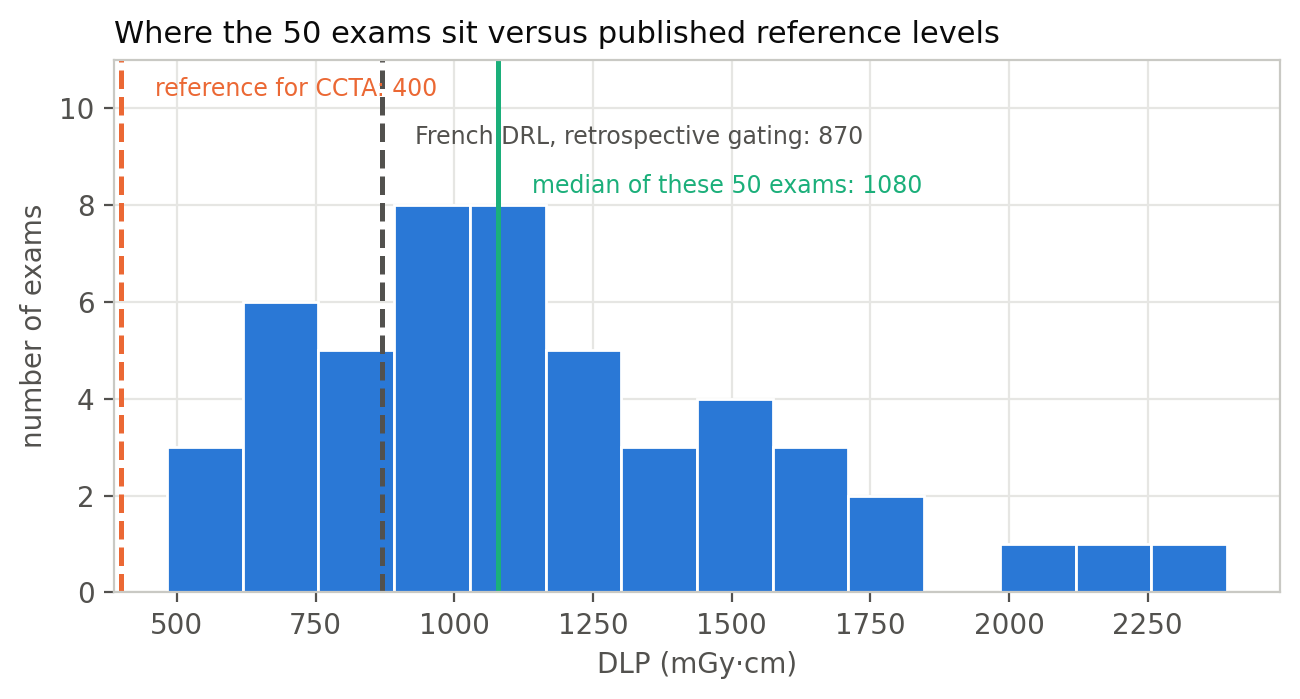
\includegraphics[width=0.98\linewidth]{figs/f4_drl.png}
\end{column}
\end{columns}
\end{frame}

% ===================== 4 DATA =====================
\begin{frame}{\kick{The data}50 exams, 7 columns --- and four findings from the audit}
\sidebar{ctblue}
\begin{columns}[T]
\begin{column}{0.46\textwidth}\scriptsize
\begin{tabularx}{\linewidth}{@{}L r r@{}}
\toprule
\hdr \textbf{Field} & \textbf{Median} & \textbf{Range}\\
\midrule
BMI (fixed) & 27.2 & 18.3--58.8\\
kVp & 120 & 120 (46) $\cdot$ 140 (4)\\
mAs & 756 & 375--1345\\
Scan size (cm) & 29.8 & 22.4--44.2\\
\ctdi{} (mGy) & 47.5 & 21.1--105\\
DLP (\mgycm) & 1080 & 482--2393\\
\bottomrule
\end{tabularx}
\vspace{2mm}
\figcap{Source: a spreadsheet printed to PDF. The app parses it directly, so re-imports need no manual typing.}
\end{column}
\begin{column}{0.52\textwidth}\footnotesize
\begin{itemize}
\item \textbf{\ctdi{} is deterministic:} 0.0605 mGy per mAs at 120~kV, 0.0894 at 140~kV --- a scanner constant,
not a correlation.
\item \textbf{``SCAN SIZE CM'' is not the scan length:} it tracks BMI ($r = 0.89$) but not DLP/CTDI ($r = -0.23$).
The implied irradiated length is $23.2 \pm 2.2$~cm.
\item \textbf{Five exams give 7\% less dose per mAs} --- a different collimation, pitch or scan mode that is not
recorded anywhere.
\item \textbf{Two pairs of duplicate rows} --- kept in the same cross-validation fold so they cannot inflate the
score.
\end{itemize}
\end{column}
\end{columns}
\end{frame}

% ===================== 5 PHYSICS =====================
\begin{frame}{\kick{The algorithm \textperiodcentered\ core}The core insight: the dose is physics, not a pattern}
\sidebar{ctblue}
\begin{columns}[T]
\begin{column}{0.42\textwidth}
\begin{eqbox}
$\ctdi = k \cdot \mathrm{mAs} \cdot (\mathrm{kVp}/120)^{n}$\\[1.5mm]
$\mathrm{DLP} = \ctdi \times \mathrm{length}$
\end{eqbox}
\vspace{1mm}
\scriptsize
\begin{itemize}
\item Fitted to this scanner: \textbf{$k = 0.0605$} mGy/mAs, \textbf{$n = 2.53$} (physics expects 2.5--3.0).
\item The \textbf{mAs exponent is fixed at 1}, not fitted --- dose is linear in tube charge. That is what lets the
model extrapolate safely.
\item Robust (Huber) fitting, so the five deviant exams do not distort the constant.
\item Everything is fitted in \textbf{log space}: the drivers multiply, they do not add.
\end{itemize}
\end{column}
\begin{column}{0.56\textwidth}
  \centering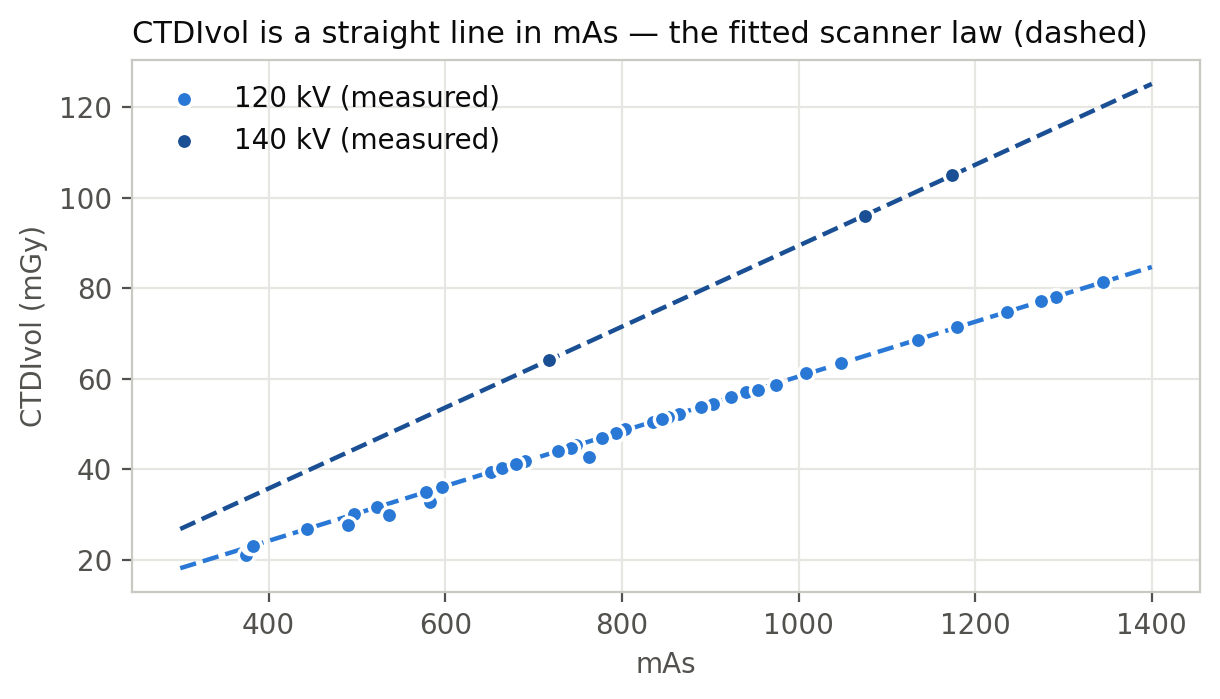
\includegraphics[width=\linewidth]{figs/f1_physics.png}\\[1mm]
  \figcap{Dashed lines are the fitted law, not a trend line through a cloud.}
\end{column}
\end{columns}
\end{frame}

% ===================== 6 ARCHITECTURE =====================
\begin{frame}{\kick{The algorithm \textperiodcentered\ architecture}One physics core, three layers}
\sidebar{ctblue}
\vspace{2mm}
\centering
\resizebox{0.96\linewidth}{!}{% Architecture diagram — shared by the report and the slides.
% Requires: tikz (arrows.meta, positioning), the ct* colours and \ctdi.
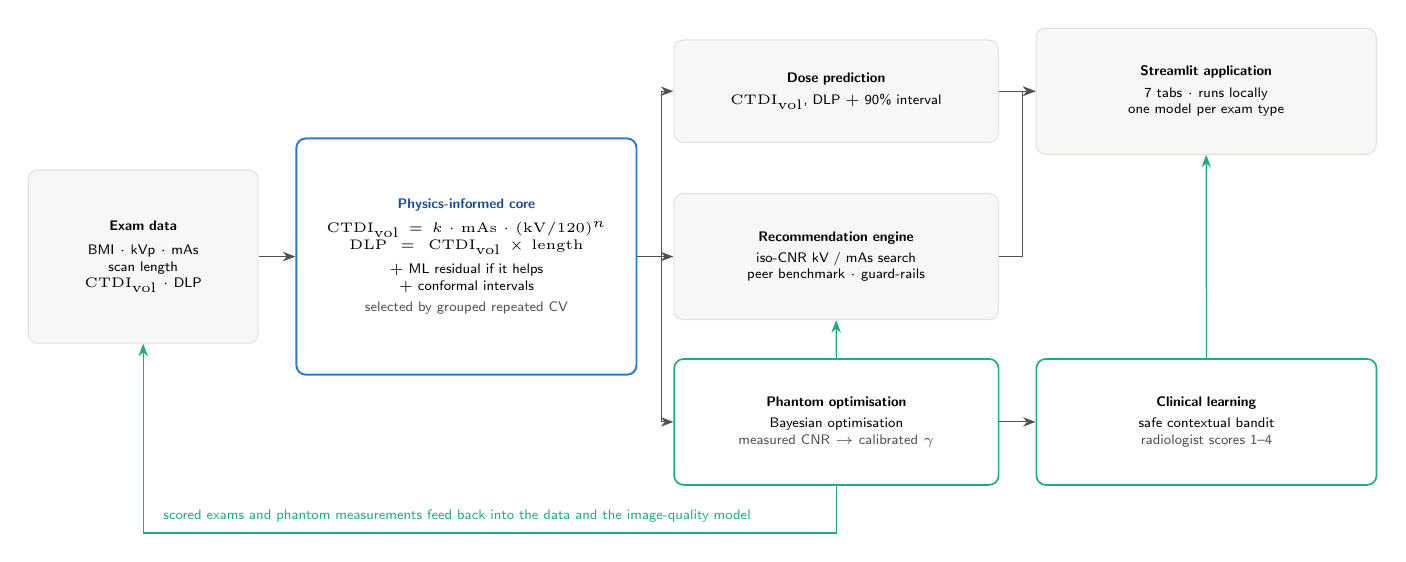
\begin{tikzpicture}[x=1mm,y=1mm,font=\sffamily\tiny,
  base/.style={rectangle,rounded corners=1.2mm,align=center,inner sep=1.6mm,anchor=west},
  box/.style={base,draw=ctline,fill=ctsurf},
  core/.style={base,draw=ctblue,line width=0.7pt,fill=white},
  loop/.style={base,draw=ctaqua,line width=0.6pt,fill=white},
  ar/.style={-{Stealth[length=1.6mm]},draw=ctink2,line width=0.35pt},
  arg/.style={-{Stealth[length=1.6mm]},draw=ctaqua,line width=0.45pt}]

\node[box,text width=26mm,minimum height=22mm] (data) at (0,0)
  {\textbf{Exam data}\\[1mm] BMI $\cdot$ kVp $\cdot$ mAs\\ scan length\\ \ctdi{} $\cdot$ DLP};

\node[core,text width=40mm,minimum height=30mm] (core) at (34,0)
  {\textbf{\textcolor{ctbluedark}{Physics-informed core}}\\[1mm]
   $\ctdi = k\cdot\mathrm{mAs}\cdot(\mathrm{kV}/120)^{n}$\\
   $\mathrm{DLP} = \ctdi \times \mathrm{length}$\\[1mm]
   $+$ ML residual if it helps\\ $+$ conformal intervals\\[0.6mm]
   {\color{ctink2}selected by grouped repeated CV}};

\node[box,text width=38mm,minimum height=13mm] (pred) at (82,21)
  {\textbf{Dose prediction}\\[0.6mm] \ctdi, DLP $+$ 90\% interval};

\node[box,text width=38mm,minimum height=16mm] (rec) at (82,0)
  {\textbf{Recommendation engine}\\[0.6mm] iso-CNR kV / mAs search\\ peer benchmark $\cdot$ guard-rails};

\node[loop,text width=38mm,minimum height=16mm] (bo) at (82,-21)
  {\textbf{Phantom optimisation}\\[0.6mm] Bayesian optimisation\\
   {\color{ctink2}measured CNR $\rightarrow$ calibrated $\gamma$}};

\node[box,text width=40mm,minimum height=16mm] (app) at (128,21)
  {\textbf{Streamlit application}\\[0.6mm] 7 tabs $\cdot$ runs locally\\ one model per exam type};

\node[loop,text width=40mm,minimum height=16mm] (band) at (128,-21)
  {\textbf{Clinical learning}\\[0.6mm] safe contextual bandit\\
   {\color{ctink2}radiologist scores 1--4}};

\draw[ar] (data.east) -- (core.west);
\draw[ar] (core.east) -- ++(3,0) |- (pred.west);
\draw[ar] (core.east) -- (rec.west);
\draw[ar] (core.east) -- ++(3,0) |- (bo.west);
\draw[ar] (pred.east) -- (app.west);
\draw[ar] (rec.east) -- ++(3,0) |- (app.west);
\draw[ar] (bo.east) -- (band.west);
\draw[arg] (bo.north) -- (rec.south);
\draw[arg] (band.north) -- (app.south);
\draw[arg] (bo.south) -- ++(0,-6) -| (data.south);
\node[font=\sffamily\tiny,text=ctaqua,anchor=west] at (16,-33)
  {scored exams and phantom measurements feed back into the data and the image-quality model};
\end{tikzpicture}
}

\vspace{3mm}
\raggedright\footnotesize\color{ctink2}
Blue = built from the supplied data. Green = the two loops that go and acquire the image-quality information the
data does not contain.
\end{frame}

% ===================== 7 BENCHMARK =====================
\begin{frame}{\kick{The algorithm \textperiodcentered\ validation}Nine models competed. Physics won --- deep learning did not.}
\sidebar{ctblue}
\centering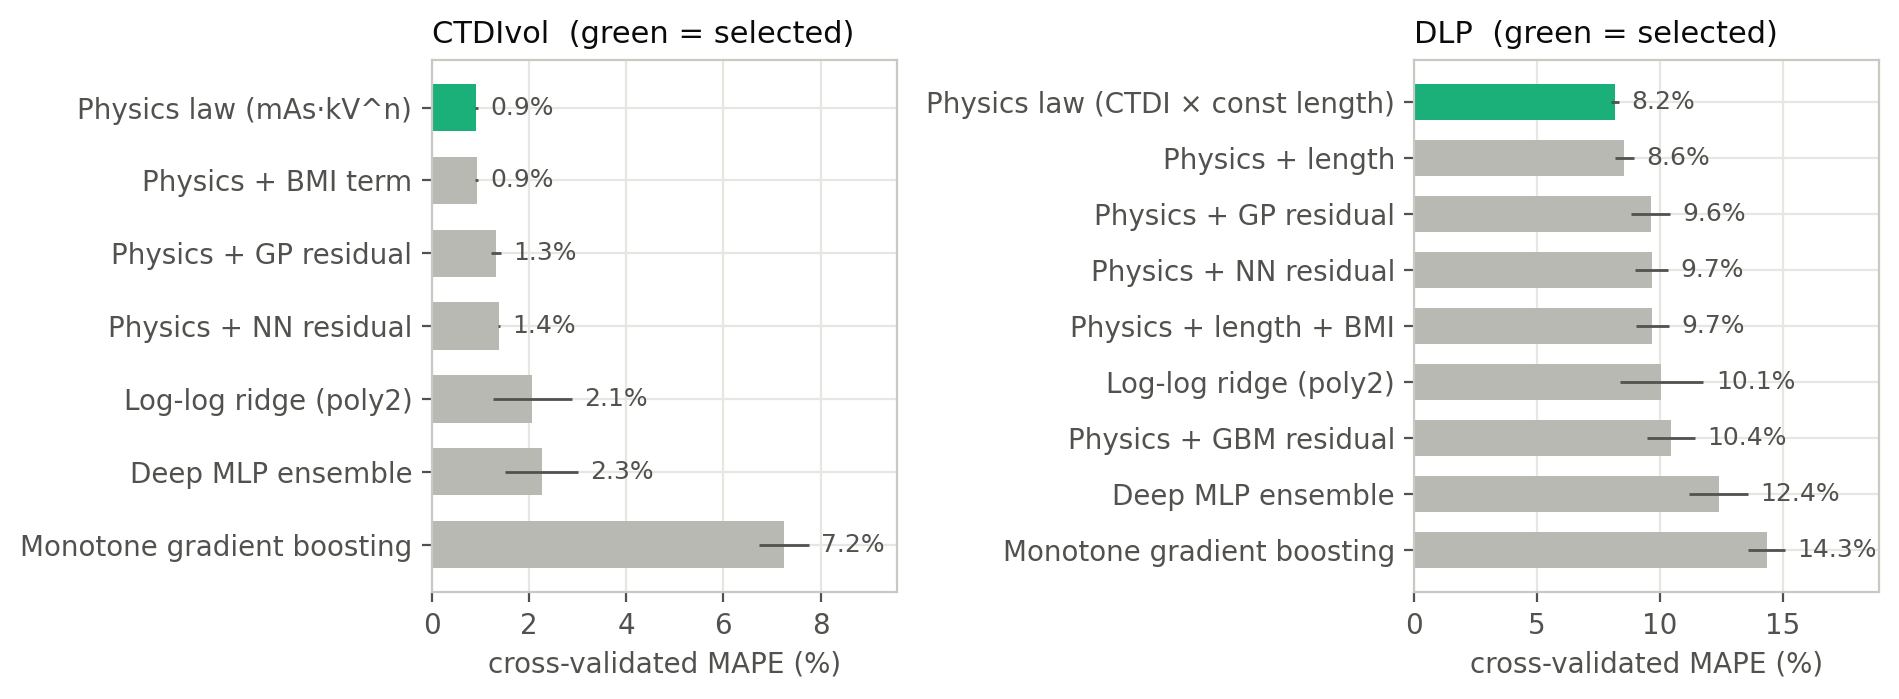
\includegraphics[width=0.90\linewidth]{figs/f2_benchmark.png}
\vspace{1mm}
\raggedright
\begin{columns}[T]
\begin{column}{0.48\textwidth}\scriptsize
\begin{itemize}
\item \textbf{Protocol:} repeated grouped 5-fold CV, 10 repeats; duplicates locked into the same fold.
\item \textbf{Selection:} 1-standard-error rule --- the simplest model within one SE of the best.
\end{itemize}
\end{column}
\begin{column}{0.48\textwidth}\scriptsize
\begin{itemize}
\item \textbf{Deep MLP ensemble:} 2.3\% and 12.4\% --- 2.5$\times$ and 1.5$\times$ worse than the physics law.
\item With 48 unique rows and a known functional form, that is the expected result, not a surprise.
\end{itemize}
\end{column}
\end{columns}
\end{frame}

% ===================== 8 WHERE ML ADDS VALUE =====================
\begin{frame}{\kick{The algorithm \textperiodcentered\ where ML actually adds value}The simple model is the answer --- the ML is everywhere else}
\sidebar{ctblue}
\begin{columns}[T]
\begin{column}{0.47\textwidth}\scriptsize
\begin{gbox}
\textbf{What machine learning contributes here}
\begin{itemize}\setlength\itemsep{1mm}
\item \textbf{An honest referee:} grouped repeated cross-validation and the 1-SE rule, so no model wins on a fluke.
\item \textbf{Calibrated uncertainty:} conformal intervals --- CTDI $\times[0.93, 1.00]$, DLP $\times[0.82, 1.25]$
at 90\%, measured coverage 94\%.
\item \textbf{Knowing its limits:} every input outside the training range is flagged, and 80/100~kV is marked as
physics extrapolation.
\item \textbf{Constrained optimisation} and \textbf{two active-learning loops} --- the parts that actually reduce
dose.
\end{itemize}
\end{gbox}
\end{column}
\begin{column}{0.51\textwidth}
  \centering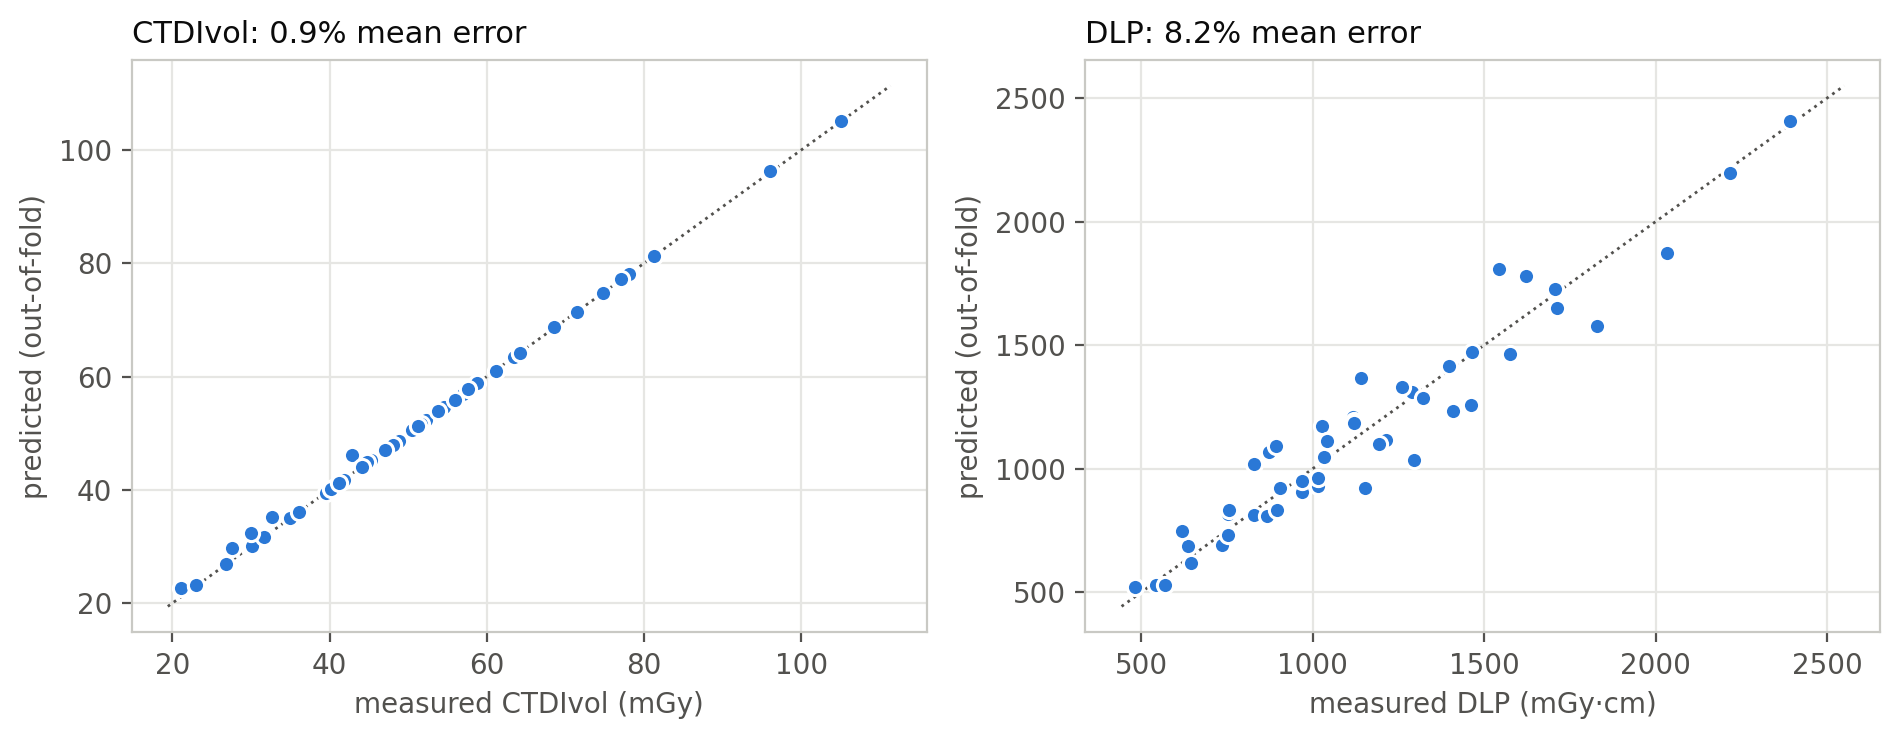
\includegraphics[width=0.98\linewidth]{figs/f3_oof.png}\\[1mm]
  \figcap{Every point predicted by a model that never saw it. The CTDI outliers are the five exams with the
  unrecorded scan mode; the DLP spread is the unrecorded scan length.}
\end{column}
\end{columns}
\end{frame}

% ===================== 9 RECOMMENDATION =====================
\begin{frame}{\kick{The solution \textperiodcentered\ recommendation engine}``What should I change?'' --- minimum dose at constant image quality}
\sidebar{ctorange}
\begin{columns}[T]
\begin{column}{0.42\textwidth}
\begin{eqbox}
noise $\propto 1/\sqrt{\ctdi}$\\[1mm]
iodine contrast $\propto \mathrm{kVp}^{-\gamma}$, $\gamma \approx 1.35$\\[1mm]
$D_{\mathrm{new}} \ge D_{\mathrm{old}}\,\tau^{2}\,(\mathrm{kV_{new}}/\mathrm{kV_{old}})^{2\gamma}$
\end{eqbox}
\footnotesize
Lower kV is the dominant lever in contrast-enhanced CT: at 100~kV the same iodine CNR needs $\approx$40\% less dose.
\vspace{2mm}
\begin{obox}\textbf{Guard-rails}
\begin{itemize}\setlength\itemsep{0.5mm}
\item Minimum kV by BMI (80 / 100 / 120)
\item Tube output limit on mAs
\item Peer benchmark from your own data
\item Length savings reported separately
\end{itemize}\end{obox}
\end{column}
\begin{column}{0.56\textwidth}
  \vspace{3mm}\centering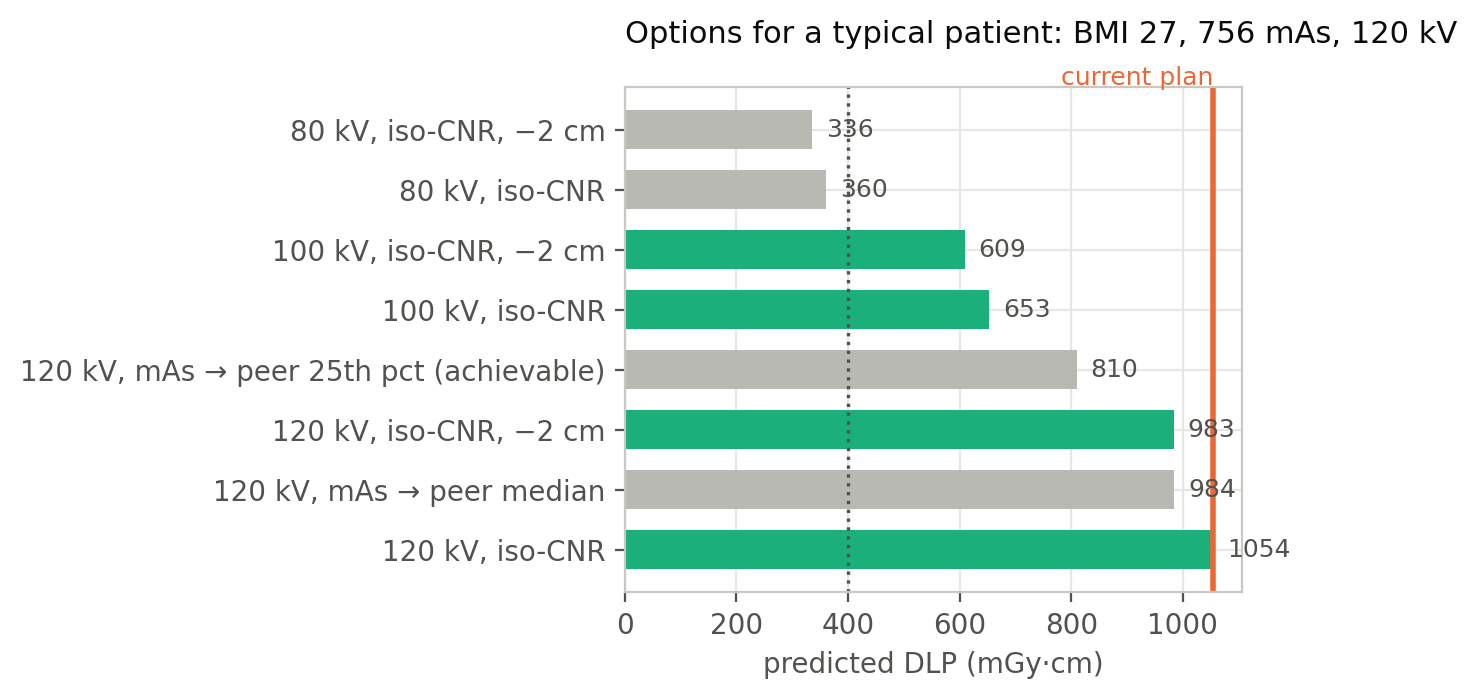
\includegraphics[width=0.96\linewidth]{figs/f5_options.png}
\end{column}
\end{columns}
\end{frame}

% ===================== 10 WORKED EXAMPLE =====================
\begin{frame}{\kick{The solution \textperiodcentered\ worked example}A typical patient: BMI 27, 120 kV, 756 mAs}
\sidebar{ctorange}
\vspace{2mm}
\kpi{$-39\%$}{\ctdi: 45.7 $\rightarrow$ 28.0 mGy}\hfill
\kpi[ctaqua]{$-42\%$}{DLP: 1056 $\rightarrow$ 609 \mgycm{} (with 2 cm less coverage)}\hfill
\kpi{100\%}{of the current estimated iodine CNR retained}\hfill
\kpi[ctorange]{100 kV}{735 mAs --- the proposed protocol}

\vspace{5mm}
\begin{columns}[T]
\begin{column}{0.48\textwidth}
\begin{cbox}\textbf{How it was derived}\\[1mm]
The mAs is raised slightly to compensate the kV drop exactly at constant iodine CNR; the dose still falls because
tube output scales as kV$^{2.53}$. Scan length acts directly on DLP.\end{cbox}
\end{column}
\begin{column}{0.48\textwidth}
\begin{obox}\textbf{What the tool says about itself}\\[1mm]
``100 kV does not appear in the training data --- this estimate relies on the fitted physics kV-law ($n = 2.53$).
Validate with a phantom or the first scans.'' The tool declares its extrapolations.\end{obox}
\end{column}
\end{columns}
\end{frame}

% ===================== 11 THE GAP =====================
\begin{frame}{\kick{The gap}But how low can we actually go?}
\sidebar{ctaqua}
{\small\color{ctink2}The data contains no information about image quality. Physics can say what keeps CNR constant;
it cannot say how much CNR is enough for a confident read. So the system goes and measures it --- in two places.\par}
\vspace{5mm}
\begin{columns}[T]
\begin{column}{0.48\textwidth}
\begin{gbox}\textbf{\normalsize 1 $\cdot$ On the phantom}\\[1.5mm]
\textbf{Bayesian optimisation.} The app proposes the next scan, you measure CNR, it proposes the next one.
Roughly 8--20 scans instead of a full grid.\\[1.5mm]
Output: the lowest-dose setting that meets your CNR target, plus a $\gamma$ calibrated on your own scanner.\end{gbox}
\end{column}
\begin{column}{0.48\textwidth}
\begin{gbox}\textbf{\normalsize 2 $\cdot$ In clinical routine}\\[1.5mm]
\textbf{Safe contextual bandit.} One proposal per patient, a radiologist approves or overrides it, then scores the
images 1--4.\\[1.5mm]
Output: the lowest dose that stays diagnostic for each BMI --- learned from your own readers, one small step at a
time.\end{gbox}
\end{column}
\end{columns}
\end{frame}

% ===================== 12 BO =====================
\begin{frame}{\kick{Learning loop 1 \textperiodcentered\ phantom}Bayesian optimisation: minimise dose subject to measured CNR}
\sidebar{ctaqua}
\begin{columns}[T]
\begin{column}{0.42\textwidth}\scriptsize
\begin{itemize}
\item \textbf{Surrogate:} $\log \mathrm{CNR} = b_0 - \gamma\log(\mathrm{kV}/120) + \delta\log \ctdi$ $+$
Gaussian-process residual, with physics priors ($\gamma \approx 1.35$, $\delta \approx 0.5$). The priors make it
useful after 2--3 scans instead of 30.
\item \textbf{Acquisition:} expected dose saving $\times$ probability of meeting the CNR target.
\item \textbf{Dose is known analytically} from the fitted scanner law, so every scan is spent on the unknown ---
image quality.
\item \textbf{Result in simulation:} the true constrained optimum after $\approx$7--8 scans, within $\sim$8\% of
it, target met in 10 of 10 runs.
\end{itemize}
\end{column}
\begin{column}{0.56\textwidth}
  \centering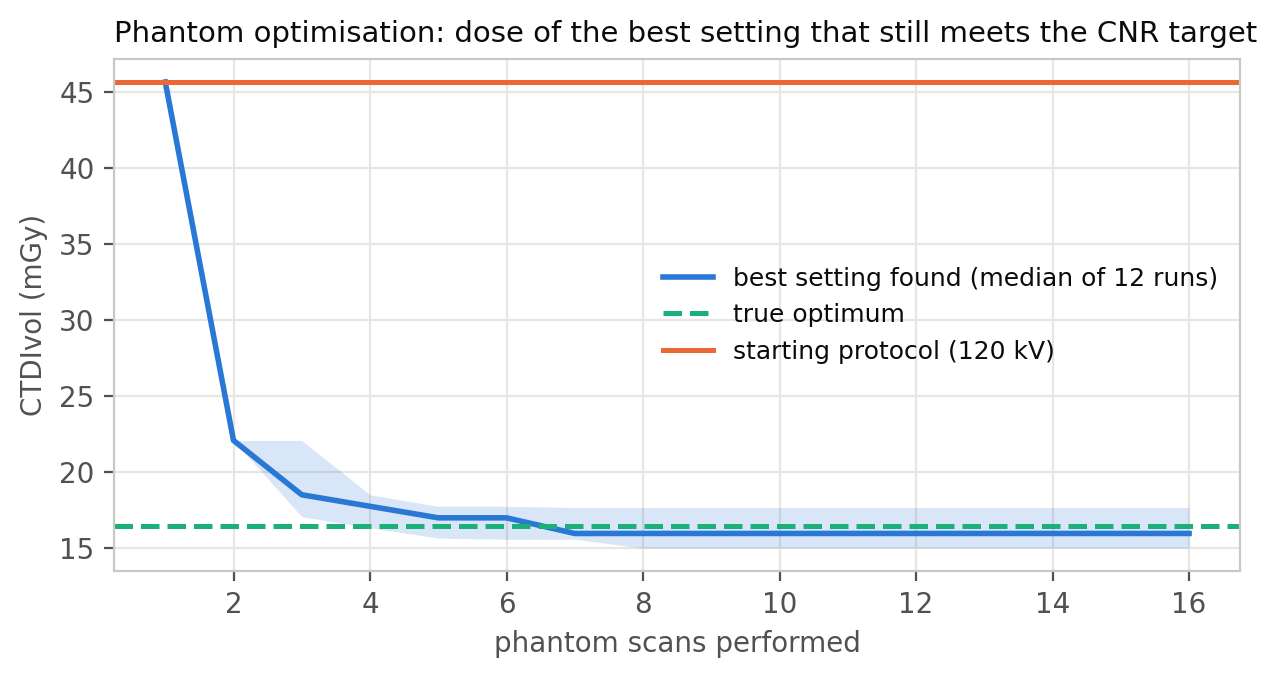
\includegraphics[width=\linewidth]{figs/f6_bo.png}\\[1mm]
  \figcap{12 simulated campaigns on a synthetic phantom; band = 10th--90th percentile.}
\end{column}
\end{columns}
\end{frame}

% ===================== 13 BANDIT =====================
\begin{frame}{\kick{Learning loop 2 \textperiodcentered\ clinical routine}A bandit that learns from radiologist scores --- under supervision}
\sidebar{ctaqua}
\begin{columns}[T]
\begin{column}{0.42\textwidth}\scriptsize
\begin{itemize}
\item \textbf{Context} BMI $\cdot$ \textbf{actions} kV $\times$ dose level $\cdot$ \textbf{reward} diagnostic score
1--4 ($\ge 3$ acceptable).
\item \textbf{Model:} Bayesian logistic regression of $P(\text{acceptable})$ on BMI, $\log$ CTDI and $\log$ kV,
with physics-informed priors. One shared model, so every exam teaches every protocol.
\item \textbf{Decision:} Thompson sampling --- the lowest-dose allowed action whose sampled $P$ clears 0.97.
Exploration shrinks by itself as evidence builds.
\item \textbf{In simulation:} $-32\%$ dose immediately, $-45$ to $-50\%$ later; 3--5\% non-diagnostic, matching the
0.97 target the department sets.
\end{itemize}
\end{column}
\begin{column}{0.56\textwidth}
  \centering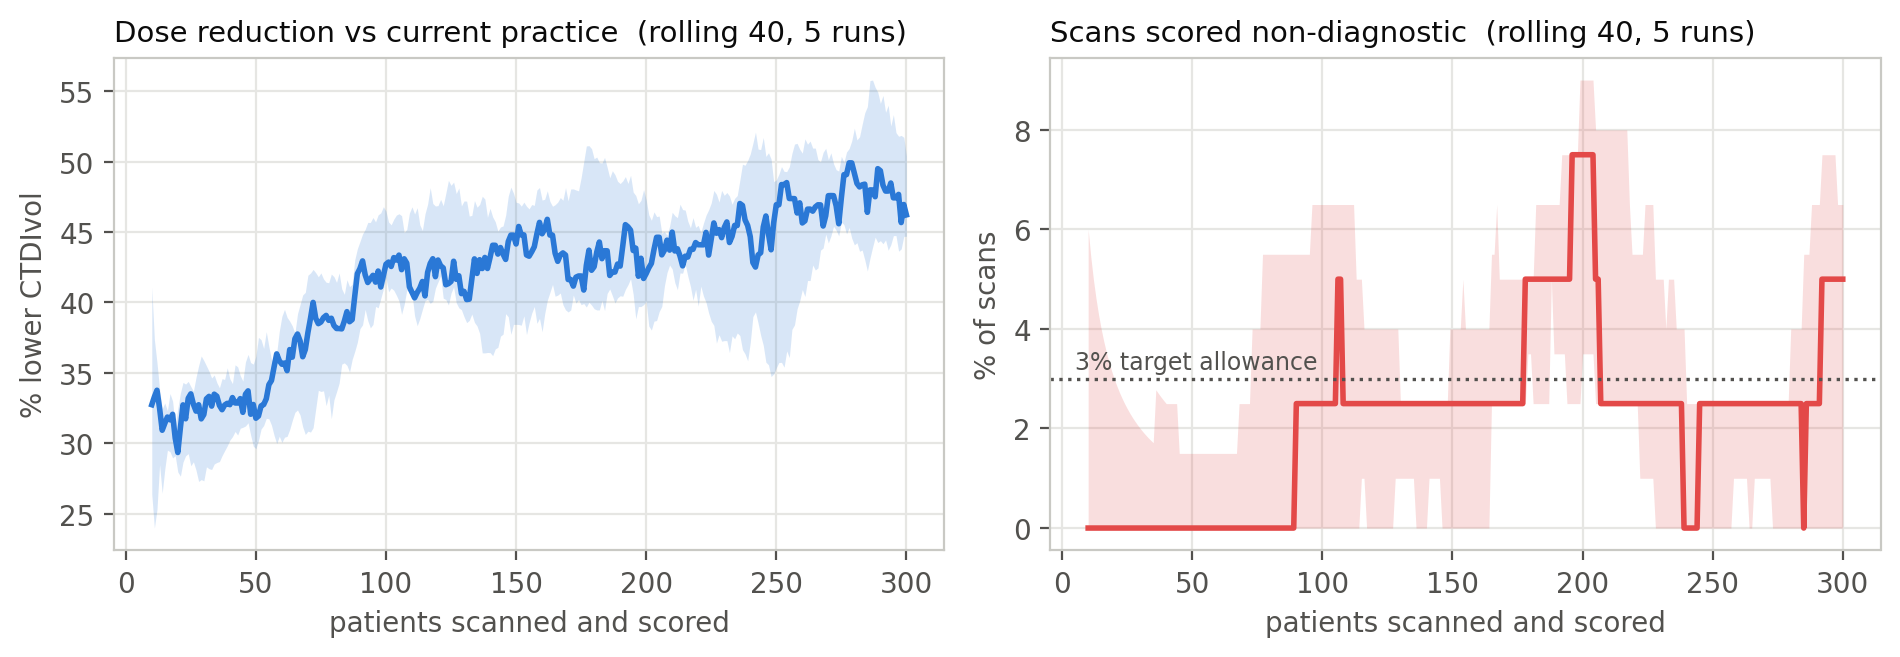
\includegraphics[width=\linewidth]{figs/f7_bandit.png}\\[1mm]
  \figcap{5 runs $\times$ 300 simulated patients with a synthetic reader; median and 10th--90th percentile.}
\end{column}
\end{columns}
\end{frame}

% ===================== 14 SAFETY =====================
\begin{frame}{\kick{Safety}Four rails, always on}
\sidebar{ctorange}
\begin{columns}[T]
\begin{column}{0.48\textwidth}
\begin{obox}\textbf{1 $\cdot$ Minimum kV by BMI}\\[1mm]
80~kV below BMI 25, 100~kV for 25--30, 120~kV above 30. No proposal can go below it --- photon starvation is never
traded for dose.\end{obox}
\vspace{2.5mm}
\begin{obox}\textbf{2 $\cdot$ Pessimistic probability floor}\\[1mm]
The 10th-percentile posterior $P(\text{acceptable})$ of a proposal must exceed 0.85. Uncertainty counts against a
protocol, never for it.\end{obox}
\end{column}
\begin{column}{0.48\textwidth}
\begin{obox}\textbf{3 $\cdot$ Small, evidenced steps}\\[1mm]
A proposal may be at most 15\% below the lowest dose already proven acceptable at a similar BMI. The dose walks
down; it never jumps.\end{obox}
\vspace{2.5mm}
\begin{obox}\textbf{4 $\cdot$ A human decides}\\[1mm]
A radiologist approves or overrides every proposal, and every override is logged. The algorithm proposes; it never
acts on its own.\end{obox}
\end{column}
\end{columns}
\vspace{3mm}
{\footnotesize\color{ctink2}Plus: out-of-domain warnings on every prediction, 13 automated tests including ``an
obese patient is never offered a sub-120~kV protocol'', and all data stays on the local machine.\par}
\end{frame}

% ===================== 15 APP =====================
\begin{frame}{\kick{The product}A local application --- seven tabs, one command to start}
\sidebar{ctblue}
\begin{columns}[T]
\begin{column}{0.40\textwidth}\scriptsize
\begin{tabularx}{\linewidth}{@{}l L@{}}
\toprule
\hdr \textbf{Tab} & \textbf{Purpose}\\
\midrule
\textbf{Predict} & dose $+$ 90\% interval, reference comparison\\
\rowcolor{ctgreenbg}\textbf{Reduce dose} & ranked options at constant CNR\\
\textbf{Phantom (BO)} & next scan to perform, calibrated $\gamma$\\
\rowcolor{ctgreenbg}\textbf{Clinical learning} & propose $\rightarrow$ approve $\rightarrow$ score $\rightarrow$ learn\\
\textbf{Batch} & whole file at once, with error report\\
\textbf{Model \& data} & model card, CV table, audit\\
\textbf{Train / add exams} & any other examination, its own model\\
\bottomrule
\end{tabularx}
\vspace{2mm}
\figcap{Runs offline on the department PC. Nothing is uploaded. \texttt{python app.py}}
\end{column}
\begin{column}{0.58\textwidth}
  \centering{\setlength{\fboxsep}{0pt}\setlength{\fboxrule}{0.4pt}\fcolorbox{ctline}{white}{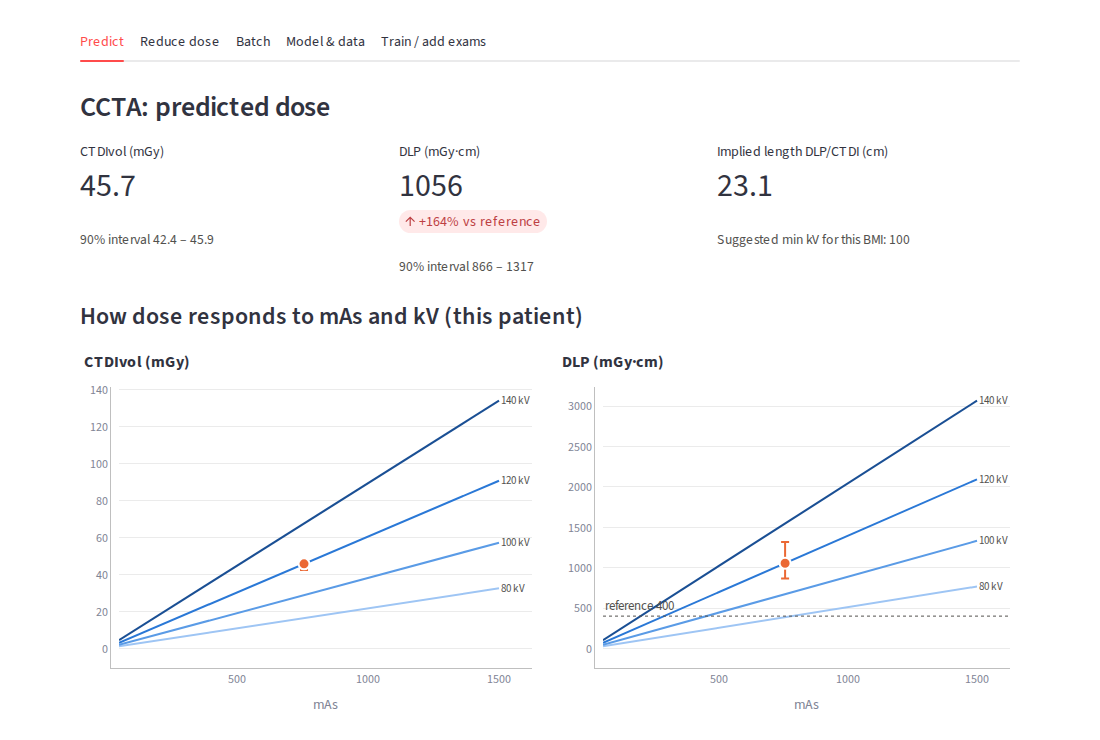
\includegraphics[width=\linewidth]{figs/app_predict.png}}}\\[1mm]
  \figcap{The Predict tab: dose with its 90\% interval, the reference-level comparison, and how dose responds to mAs
  at each kV for this patient.}
\end{column}
\end{columns}
\end{frame}

% ===================== 16 CLOSING THE LOOP =====================
\begin{frame}{\kick{The system}Every scan makes the next one better}
\sidebar{ctaqua}
\vspace{2mm}
\begin{columns}[T]
\begin{column}{0.315\textwidth}
\begin{cbox}\textbf{\color{ctbluedark}1 $\cdot$ Phantom $\rightarrow$ engine}\\[1mm]
The campaign measures $\gamma$ on your scanner, and it replaces the literature value in the recommendation engine
and in the bandit's action set.\end{cbox}
\end{column}
\begin{column}{0.315\textwidth}
\begin{cbox}\textbf{\color{ctbluedark}2 $\cdot$ Readers $\rightarrow$ engine}\\[1mm]
Each scored exam updates the acceptability model. ``Reduce dose'' then shows the lowest dose \textit{proven}
acceptable at that BMI --- local evidence, not assumption.\end{cbox}
\end{column}
\begin{column}{0.315\textwidth}
\begin{cbox}\textbf{\color{ctbluedark}3 $\cdot$ Console $\rightarrow$ dataset}\\[1mm]
Scored exams with console doses are appended to the training data. The next training run re-runs the full model
competition on more data.\end{cbox}
\end{column}
\end{columns}
\vspace{6mm}
\begin{gbox}\normalsize The dataset that started as 50 rows in a PDF grows by itself through routine use --- and if
a flexible model ever starts winning the competition, the pipeline will select it automatically.\end{gbox}
\end{frame}

% ===================== 17 RESULTS =====================
\begin{frame}{\kick{Results}Where we stand}
\sidebar{ctblue}
\scriptsize
\begin{tabularx}{\linewidth}{@{}L l L@{}}
\toprule
\hdr \textbf{Question} & \textbf{Answer} & \textbf{Evidence}\\
\midrule
\rowcolor{ctgreenbg}Predict \ctdi? & Yes --- 0.9\% error, R\textsuperscript{2} 0.998 & repeated grouped CV, 50 exams\\
\rowcolor{ctgreenbg}Predict DLP? & Yes --- 8.2\% error, R\textsuperscript{2} 0.92 & limited by the unrecorded scan length\\
Does deep learning help? & No --- 2.3\% and 12.4\% & identical protocol for all nine models\\
Say what to change? & Yes --- ranked options at constant CNR & iso-CNR physics $+$ guard-rails\\
How much dose could go? & $\approx$40\% at 100 kV, $\approx$65\% at 80 kV (slim) & physics estimate, phantom to confirm\\
Find the optimum experimentally? & Yes --- $\approx$8 phantom scans & 12 simulated campaigns\\
Keep learning safely in routine? & Yes, with approval at every step & 1500 simulated patients\\
\bottomrule
\end{tabularx}
\vspace{3mm}
\begin{obox}\textbf{What the simulations prove:} that the algorithms converge, respect their constraints and behave
safely. \textbf{What they do not prove:} clinical benefit. The real numbers depend on your scanner, your
reconstruction and your readers --- which is what the phantom campaign and the pilot are for.\end{obox}
\end{frame}

% ===================== 18 ASKS =====================
\begin{frame}{\kick{What we need}Five questions for the data provider}
\sidebar{ctblue}
\small
\begin{itemize}\setlength\itemsep{2.2mm}
\item \textbf{What exactly is ``SCAN SIZE CM''?} It tracks BMI, not the irradiated length. The true $z$-coverage
should take DLP error from $\sim$8\% towards $\sim$1\%.
\item \textbf{What differs in rows 2, 9, 22, 41, 45?} They deliver 7\% less dose per mAs --- probably collimation,
pitch or scan mode.
\item \textbf{Are rows 28/43 and 29/42 really two patients each?} They are identical in every field.
\item \textbf{Is the protocol retrospectively gated?} If prospective triggering is feasible at the patient's heart
rate, it saves more than any kV or mAs change --- but it is outside the four parameters we were given.
\item \textbf{Which fields can be exported routinely?} Scan length $\cdot$ gating mode $\cdot$ collimation and
pitch $\cdot$ heart rate $\cdot$ reconstruction level $\cdot$ a 1--4 diagnostic-quality score.
\end{itemize}
\end{frame}

% ===================== 19 ROADMAP =====================
\begin{frame}{\kick{Next steps}From 50 rows in a PDF to a department-wide tool}
\sidebar{ctaqua}
\scriptsize
\begin{tabularx}{\linewidth}{@{}l L L@{}}
\toprule
\hdr \textbf{Stage} & \textbf{Action} & \textbf{Outcome}\\
\midrule
\textbf{1 $\cdot$ Data} & Export the extra fields for existing exams and the next 100--200 cases & DLP error towards 1--2\%\\
\rowcolor{ctgreenbg}\textbf{2 $\cdot$ Phantom} & One campaign with the physicist: 10--20 scans, entering measured CNR & Site-specific $\gamma$, evidence-based low-kV protocol\\
\textbf{3 $\cdot$ Pilot} & 20--30 patients at the phantom-derived protocol, each scored 1--4 & First real acceptability data; go / no-go\\
\rowcolor{ctgreenbg}\textbf{4 $\cdot$ Routine} & Clinical-learning loop on conservative settings & Gradual, evidenced dose reduction\\
\textbf{5 $\cdot$ Expansion} & Brain, chest, abdomen --- each gets its own model & Department dose-optimisation platform\\
\bottomrule
\end{tabularx}
\vspace{7mm}

{\large\bfseries Thank you}\\[1.5mm]
{\footnotesize\color{ctink2}Questions, and the phantom slot, are the next step.\\
github.com/Thodoris1657/CT-Dose-AI-Algorithm\par}
\hfill
\end{frame}

\end{document}
